%!TEX root = ../thesis.tex

% \vspace{-10pt}

% \section{本章の概要}
本章では,移動ロボットのナビゲーションにおける予測結果の活用方法を検討するための実験を実施し,その結果を評価する.
また,実験では指定した軌道を往復する人のモデルを対象に,予測された歩行者の軌道をどのように活用できるかを議論する.
まず,実験の概要について説明し,次に実験シナリオと使用したシミュレータ環境について述べる.最後に,実験結果を踏まえて考察を行う.

\section{実験概要}
予測結果を応用したナビゲーションシステムによって,移動ロボットの挙動がどのように変化するかを観察・評価するための実験を行った.実験では,3つのナビゲーションシナリオを設定し,移動ロボットを自律走行させる.なお,各シナリオにつき10回ずつ走行を実施してデータを取得した.

% \section{実験方法}
本実験の予測には,\ref{chap:proposed_method}章で提案したネットワークを用いた.ただし,使用したモデルはホールドアウト(Hold Out)方式で学習を行った.それ以外は同様の学習条件である.
さらに,\ref{chap:application}章で述べたシステムを用いて,ナビゲーションに予測結果を適用した.
\newpage
実験は\figref{Fig:sim-env}に示すように,Gazebo\cite{Gazebo62:online}のシミュレータ環境上で行った.また,\figref{Fig:sim-robot}に示すように,シミュレータで再現した移動ロボット(ORNE-box2\cite{井口颯人2023屋外自律移動ロボットプラットフォーム-orne})を用い,\figref{Fig:sim-actor}に示す歩行者はGazeboのプラグイン\cite{Actors-G87:online}を使用してシミュレータ内に配置した.歩行者の動きには,Social Force Model\cite{s-force-model}に基づくプラグイン\cite{techlife87:online-sfm-plugin}を用いており,パラメータは歩行速度のみを$0.6m/s$に変更して実験を行った.

\begin{figure}[H]
  \centering
 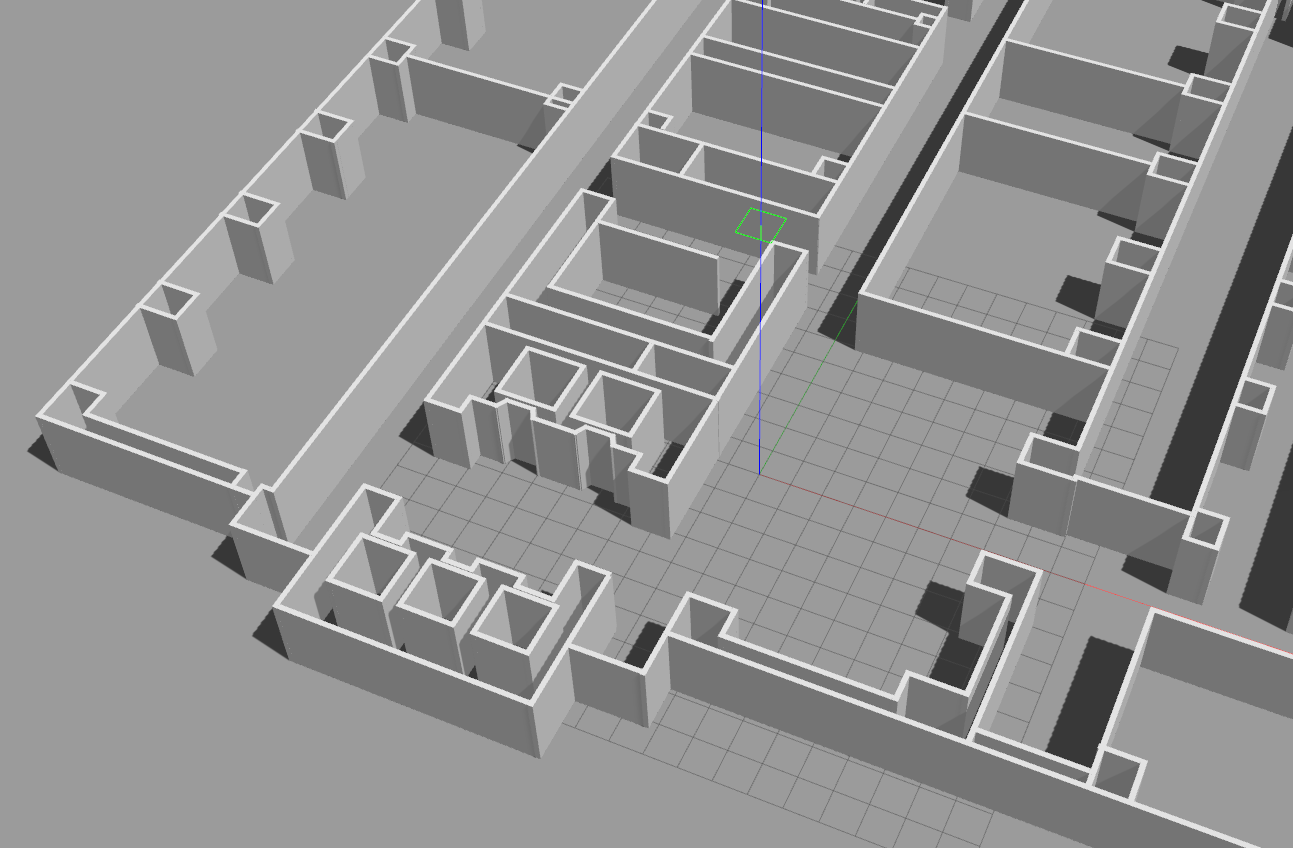
\includegraphics[keepaspectratio, scale=0.15]
      {images/sim-env.png}
\caption{Simulator environment}
 \label{Fig:sim-env}
\end{figure} 

\vspace{-10pt}

\begin{figure}[H]
  \centering
  \begin{subfigure}{0.40\textwidth}
    \centering
    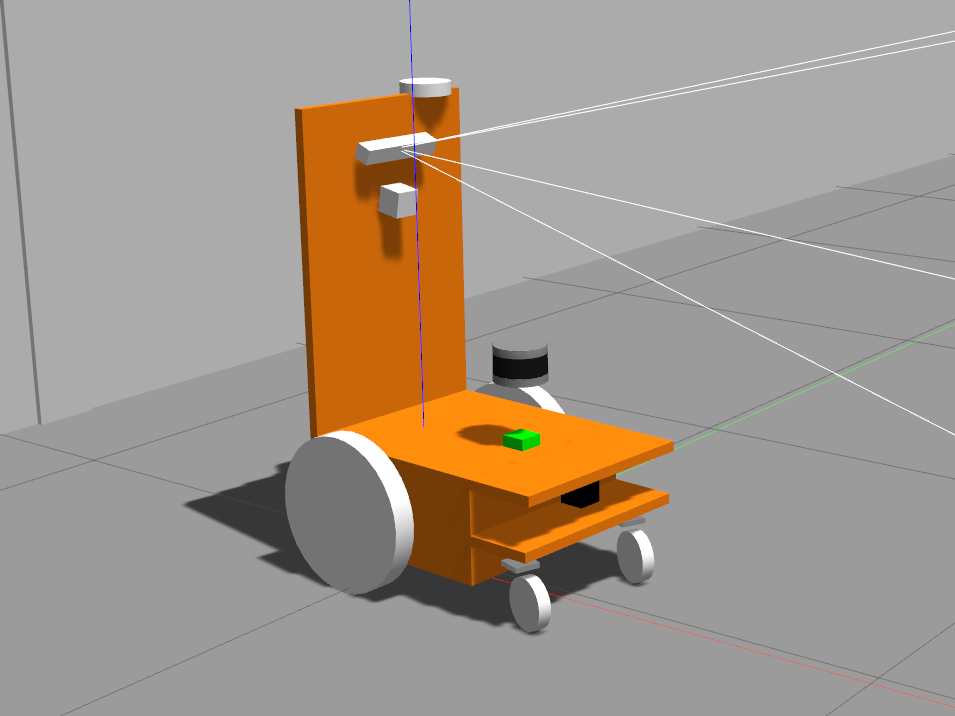
\includegraphics[keepaspectratio, scale=0.15]{images/sim-robot.png}
    \caption{Simulated robot}
    \label{Fig:sim-robot}
  \end{subfigure}
  % \hfill
  \begin{subfigure}{0.40\textwidth}
    \centering
    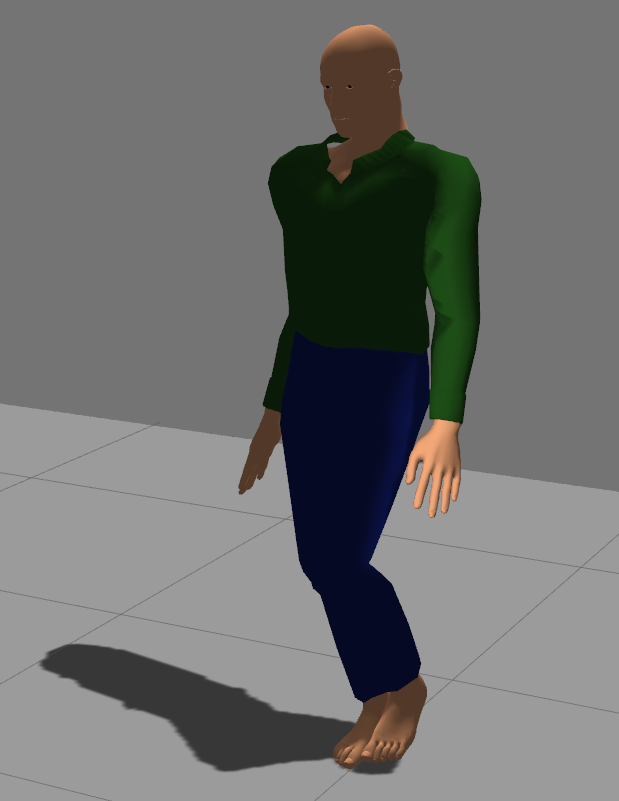
\includegraphics[keepaspectratio, scale=0.15]{images/sim-actor.png}
    \caption{Simulated actor}
    \label{Fig:sim-actor}
  \end{subfigure}
  \caption{Simulated robot and actor}
  \label{Fig:sim-robot-actor}
\end{figure}

% 移動ロボットの自律走行は,つくばチャレンジ2024EX@イーアスつくば\cite{つくばチャレンジ36:online}で千葉工業大学 未来ロボティクス学科 box2チームが完走した際のソフトウェア構成,パラメータを参考にした.これは,Githubで公開されている\cite{openrdco85:online}.なお,後述するシナリオには狭い通路の走行が含まれるため,yaw方向の角速度を小さくなるように変更している.

本研究で用いた移動ロボットの自律走行ソフトウェアおよびパラメータ設定は,つくばチャレンジ2024EX@イーアスつくば\cite{つくばチャレンジ36:online}において,千葉工業大学 未来ロボティクス学科 box2チームが完走した際の構成を参考にしている(Github\cite{openrdco85:online}で公開).なお,後述のシナリオには狭い通路を走行する箇所が含まれているため,yaw方向の角速度を小さくしている.

\newpage

% 実験は以下に示す3種類のシナリオで行った.
% \figref{Fig:scenario1}のシナリオ1では,ロボットが直線経路を進む途中に歩行者が横断する状況を設定した.
% \figref{Fig:scenario2}のシナリオ2では,ロボットが狭い通路で正面から近づく歩行者とすれ違う状況を設定した.
% \figref{Fig:scenario3}のシナリオ3では,ロボットが狭い通路を走行する際に2名の歩行者がすれ違う状況を設定し,より複雑な環境下でのナビゲーションを想定している.

本実験は,以下の3つのシナリオで行った.
\begin{itemize}
  \vspace{-10pt}
  \item \textbf{シナリオ1}(\figref{Fig:scenario1})\\
  ロボットが直線経路を走行中に,歩行者が横断する状況を設定した.
  \item \textbf{シナリオ2}(\figref{Fig:scenario2})\\
  ロボットが狭い通路で正面から接近する歩行者とすれ違う状況を設定した.
  \item \textbf{シナリオ3}(\figref{Fig:scenario3})\\
  ロボットが狭い通路を走行する際に2名の歩行者がすれ違う状況を設定し,より複雑な環境下でのナビゲーションを想定している.
\end{itemize}

\vspace{-5pt}

\begin{figure}[H]
  \centering
  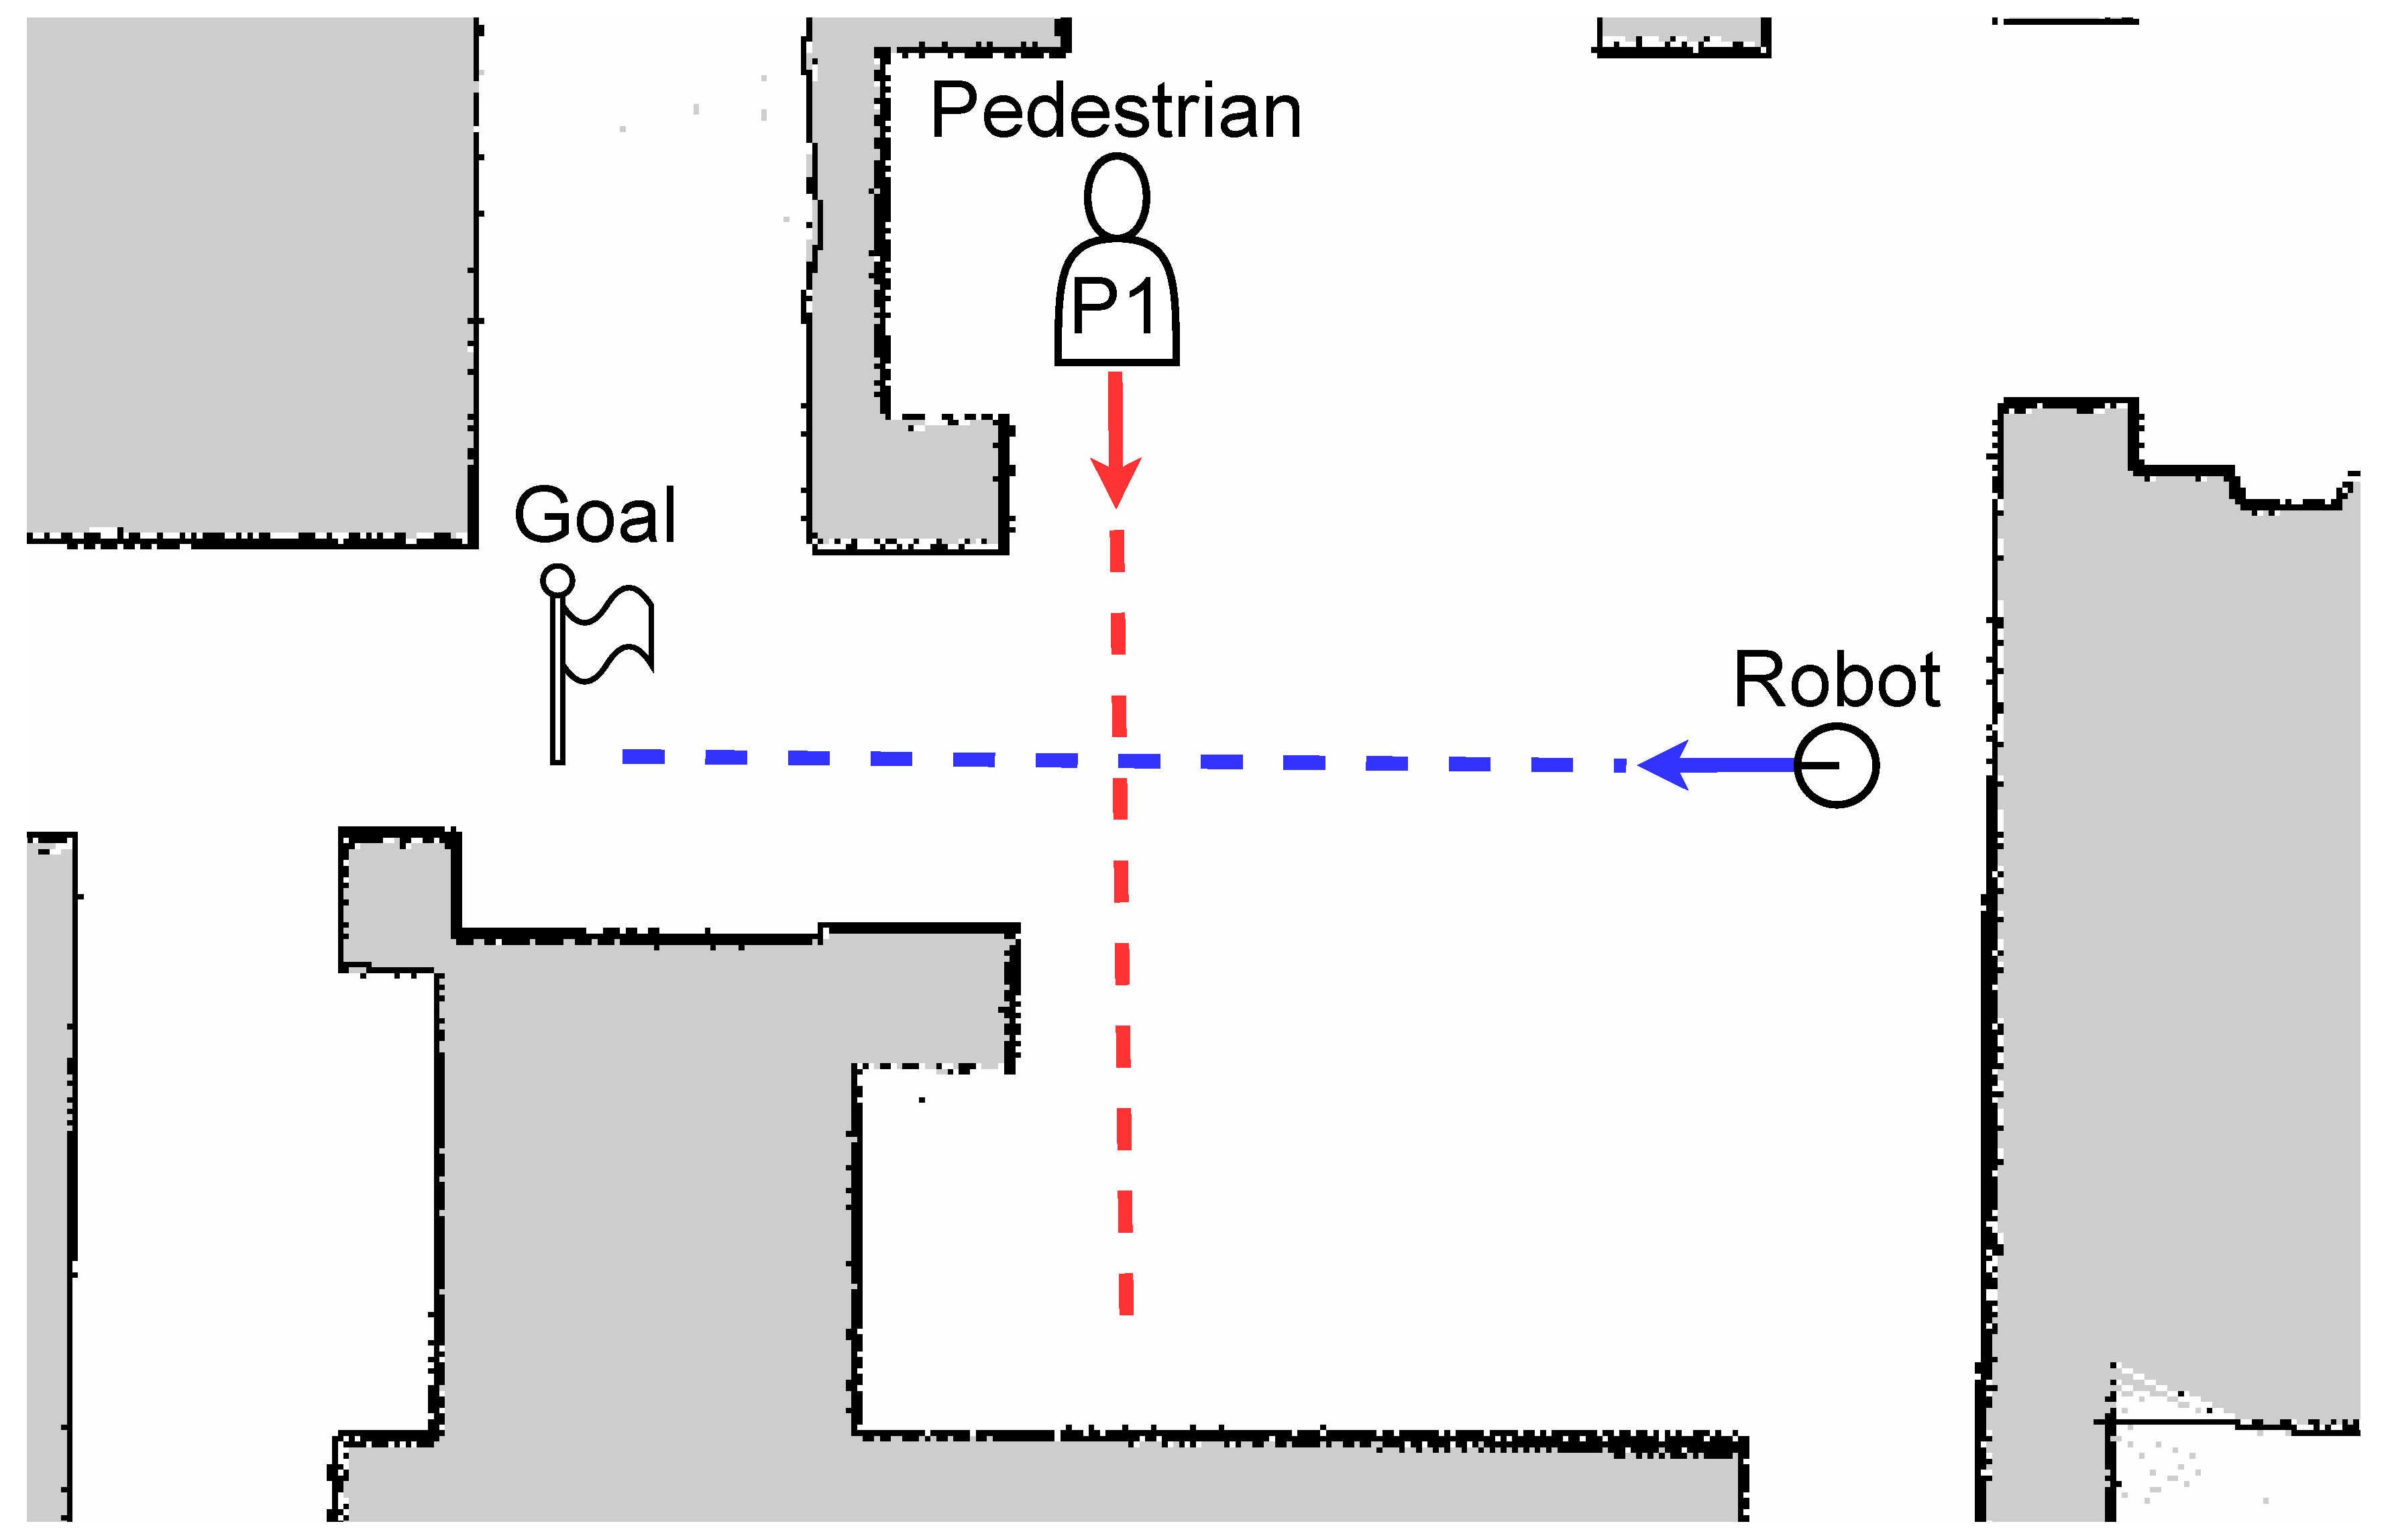
\includegraphics[keepaspectratio, scale=0.15]{images/scenario1.pdf}
  \caption{Experiment scenario 1}
  \label{Fig:scenario1}
\end{figure}

\vspace{-20pt}

\begin{figure}[H]
  \centering
  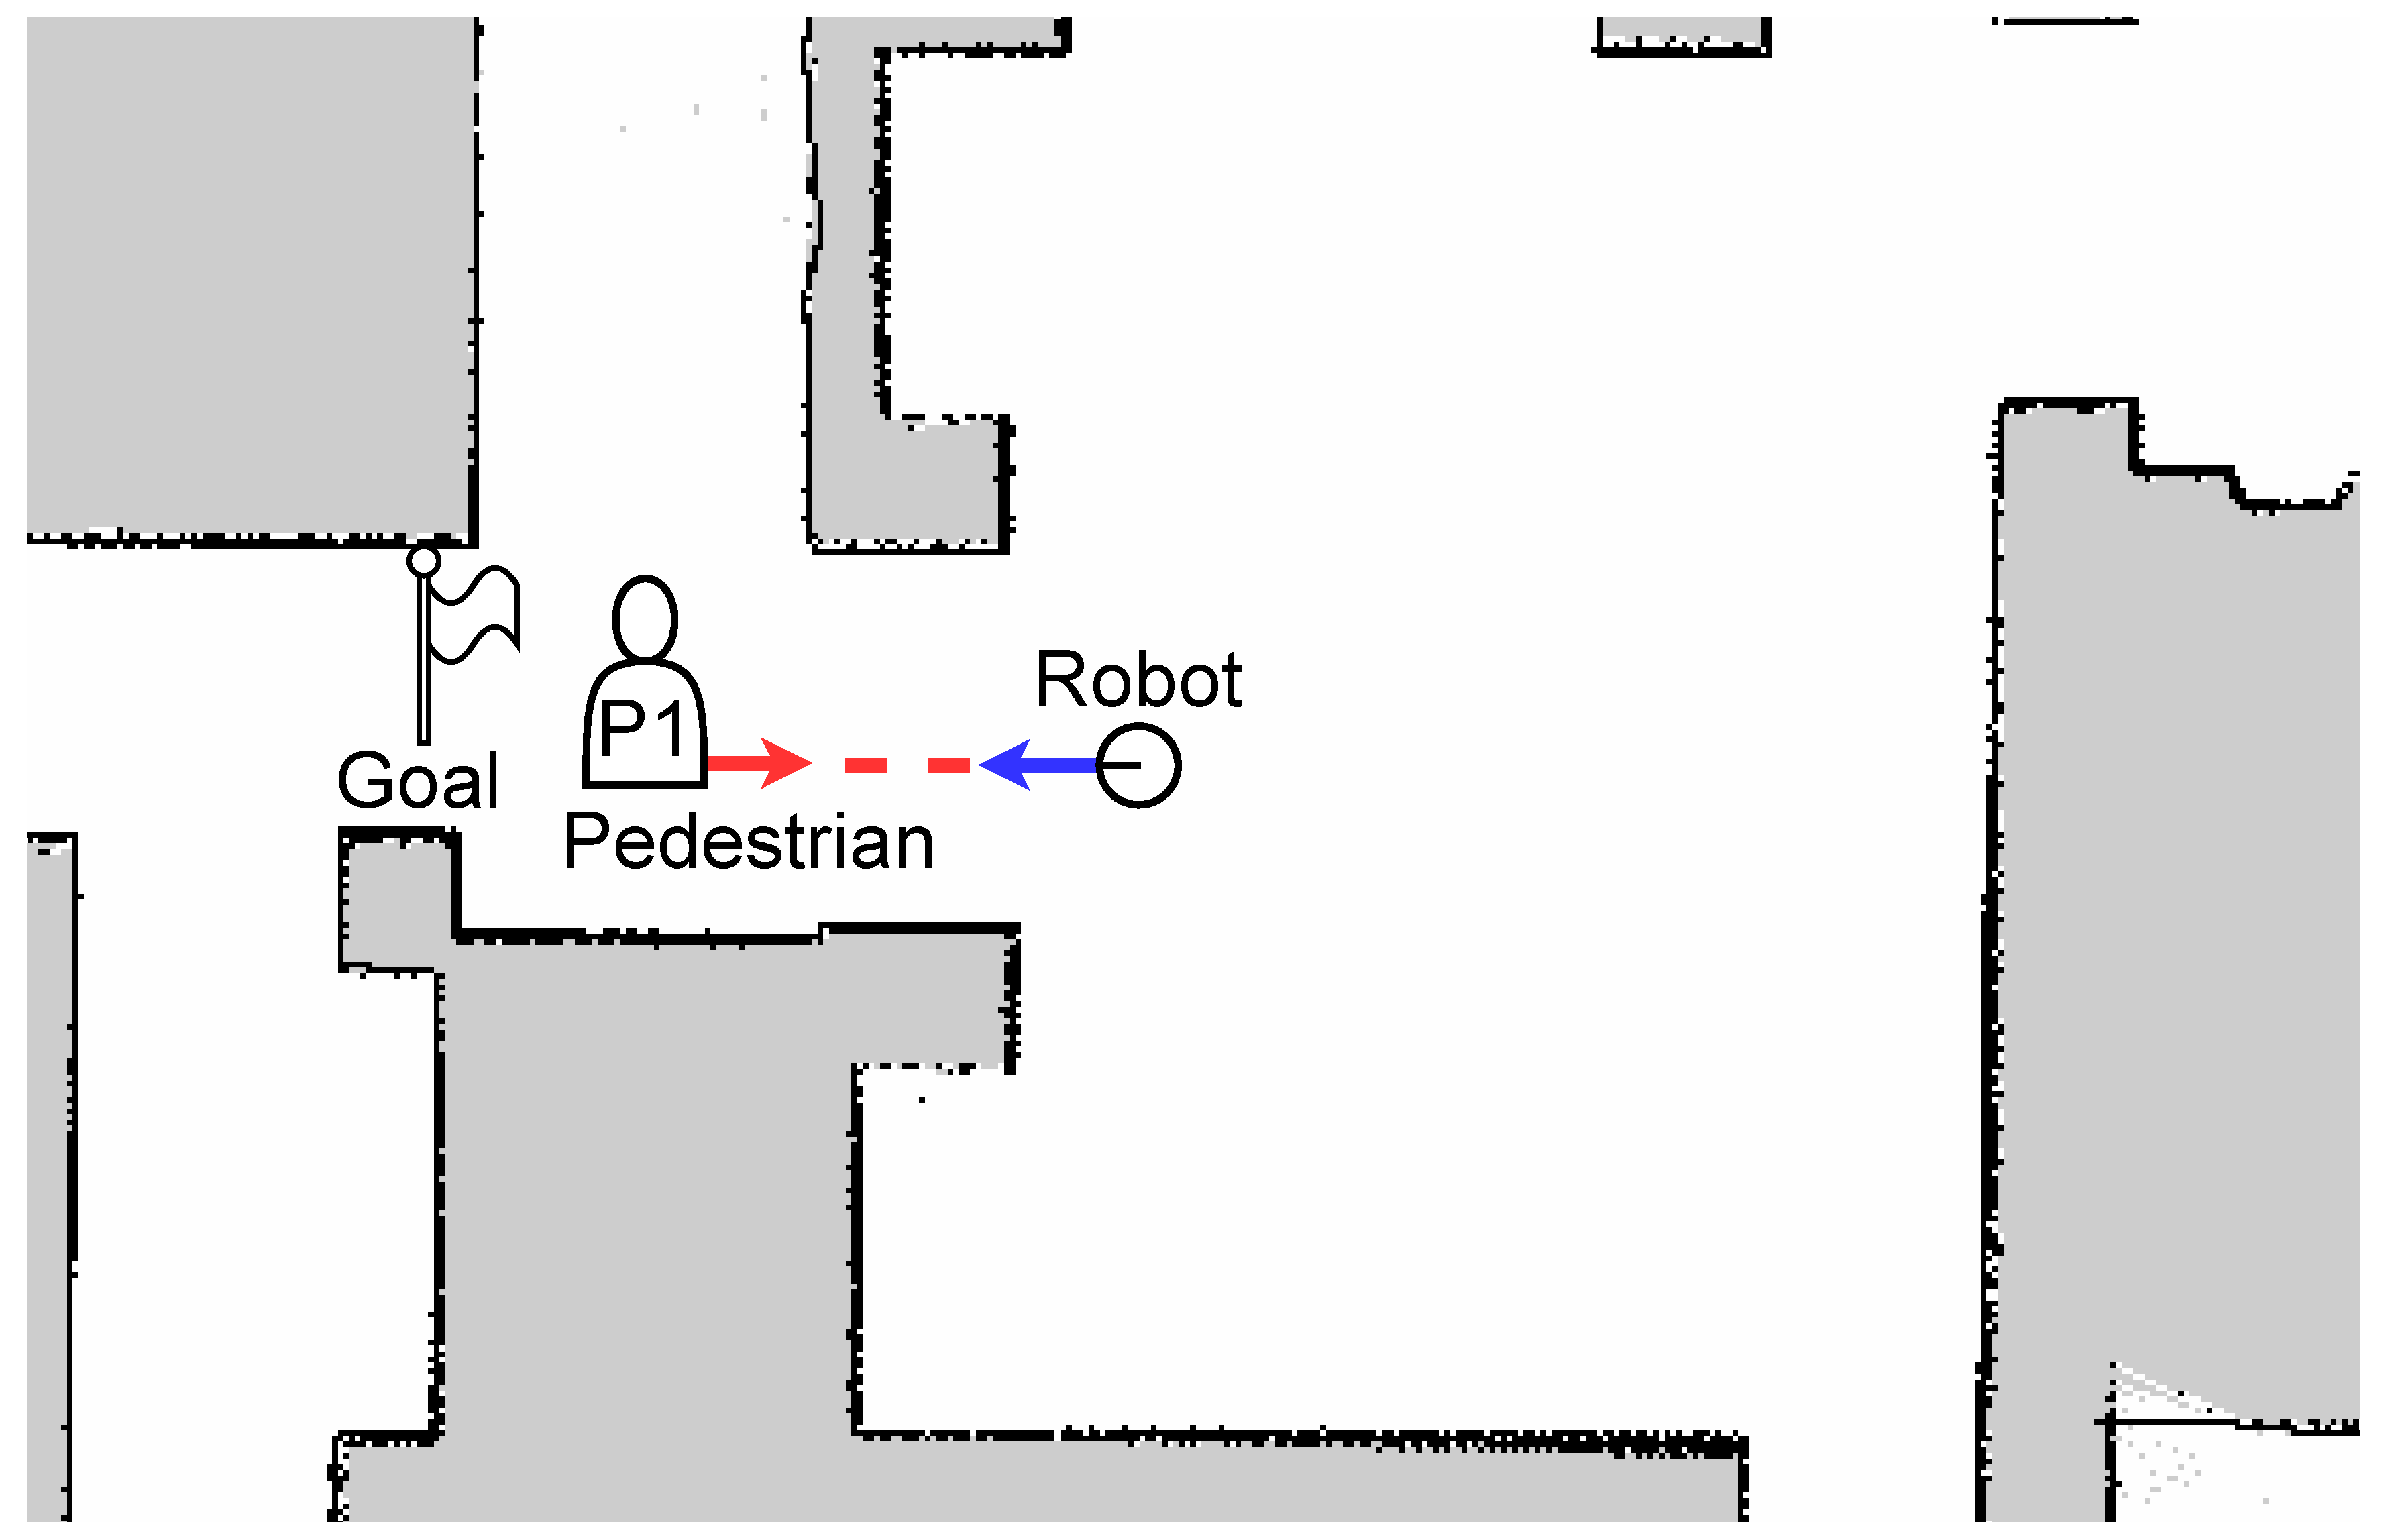
\includegraphics[keepaspectratio, scale=0.15]{images/scenario2.pdf}
  \caption{Experiment scenario 2}
  \label{Fig:scenario2}
\end{figure}

\begin{figure}[H]
  \centering
  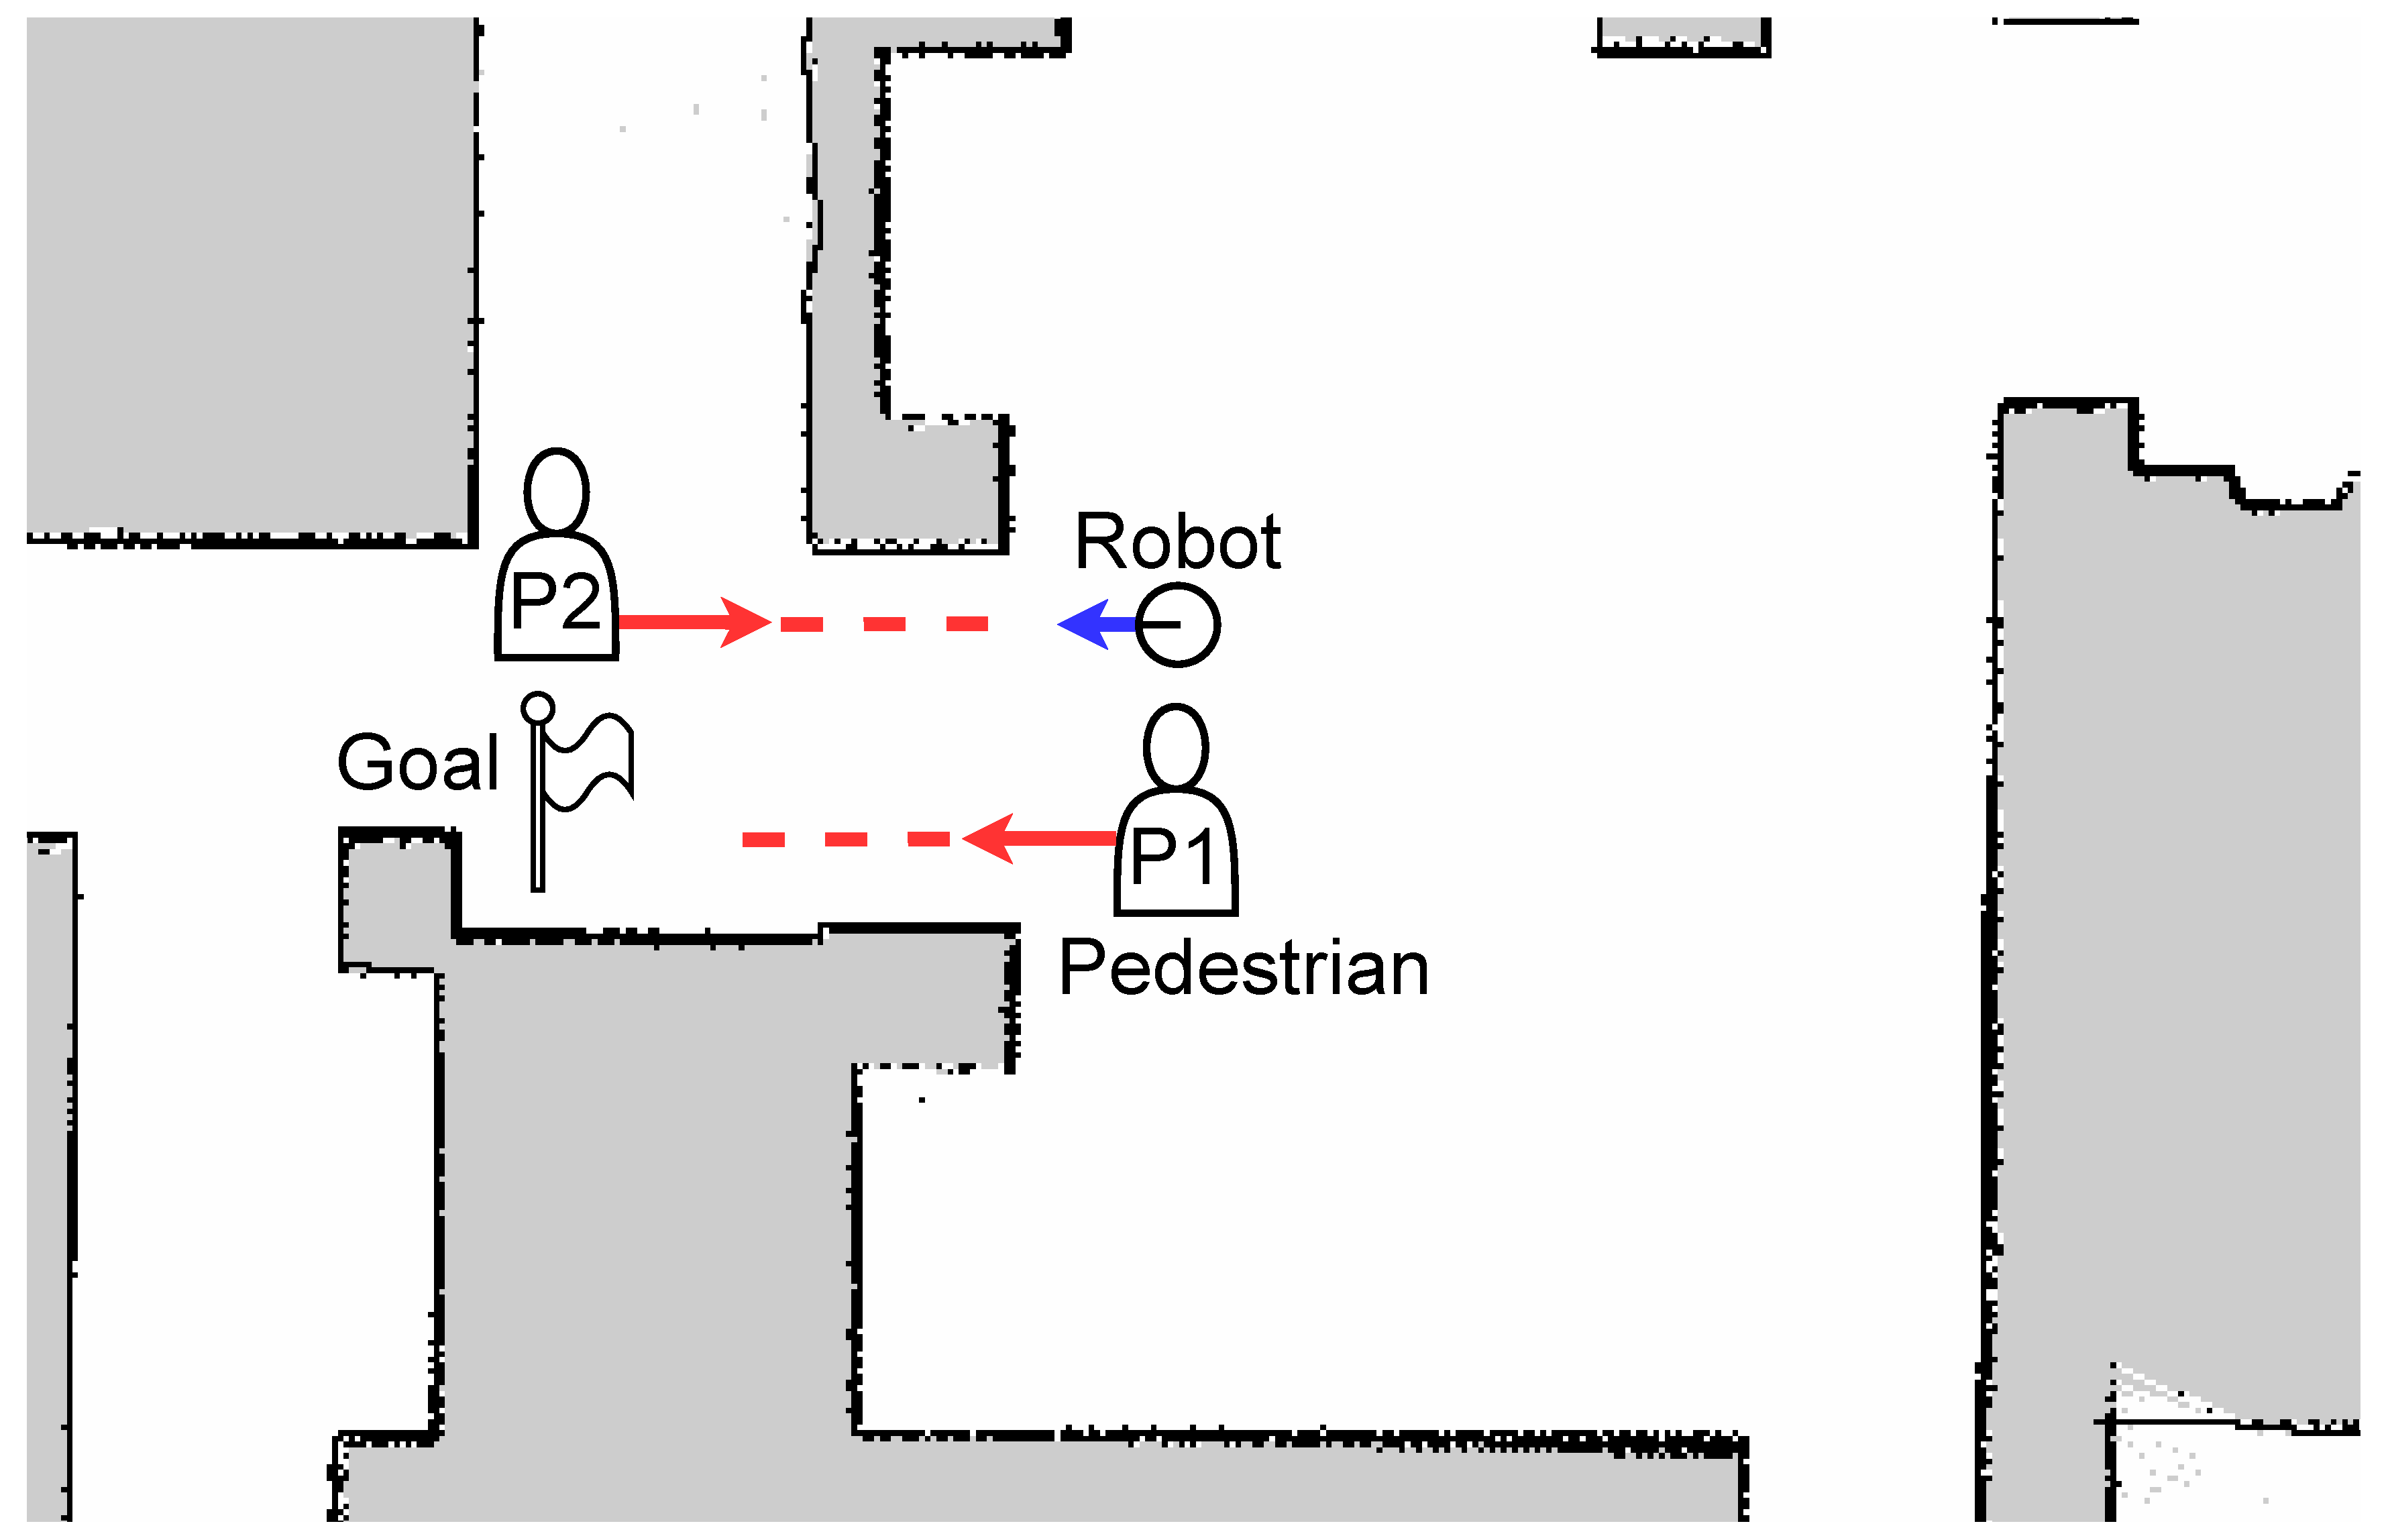
\includegraphics[keepaspectratio, scale=0.15]{images/scenario3.pdf}
  \caption{Experiment scenario 3}
  \label{Fig:scenario3}
\end{figure}

% \newpage

評価は以下の4項目に基づいて行った.
\begin{itemize}
  \item 走行時間
  \item 走行距離
  \item 歩行者とロボット間の最小距離
  \item 最小のTime to Collision(TTC)
\end{itemize}
% ナビゲーションの効率性は走行時間・距離が小さいほど高く,人間とロボット間の接触リスクは最小距離・最小TTCが大きいほど少ないと考えられる.

ナビゲーションの効率性は,一般的に走行時間および走行距離が小さいほど高いと考えられる.しかし,この評価は具体的な状況や環境条件に依存する可能性がある.一方で,人間とロボット間の接触リスクは,最小距離および最小TTCが大きいほど低減されると考えられる.
TTCは,移動物体同士が現在の速度と進行方向を維持した場合の衝突するまでの時間を示し,以下の式で計算される.
\setlength{\jot}{1em}
\begin{align}
  \mathbf{v}_{\text{robot}} = \begin{bmatrix} v_{\text{robot}x} \\ v_{\text{robot}y} \end{bmatrix}, \quad 
  \mathbf{v}_{\text{ped}} &= \begin{bmatrix} v_{\text{ped}x} \\ v_{\text{ped}y} \end{bmatrix} \\
  \mathbf{v}_{\text{relative}} &= \mathbf{v}_{\text{robot}} - \mathbf{v}_{\text{ped}} \\
  \text{TTC} &= \frac{d}{\|\mathbf{v}_{\text{relative}}\|}
\end{align}
ここで,$d$はロボットと歩行者の距離,$\mathbf{v}_{\text{robot}}$はロボットの速度ベクトル,$\mathbf{v}_{\text{ped}}$は歩行者の速度ベクトルである.

\section{結果と考察}\label{sec:exp-sim-result}
\figref{Fig:scenario1-result},\figref{Fig:scenario2-result},\figref{Fig:scenario3-result}は,各シナリオにおいて予測結果を用いないナビゲーションとロボットの行動を考慮した予測結果を用いるナビゲーションの比較結果である.棒グラフは平均値,エラーバーは標準偏差を表す.

まず,\figref{Fig:scenario1-result}に示すシナリオ1の結果を比較すると,走行時間が約78%,走行距離が約3%悪化した一方で,最小距離が約29%,最小TTCが約55%改善した.
次に,\figref{Fig:scenario2-result}に示すシナリオ2の結果では,走行時間が約54%,走行距離が約4%悪化したが,最小距離が約10%,最小TTCが約14%改善した.
また,\figref{Fig:scenario3-result}に示すシナリオ3の結果では,走行時間が約57%,歩行者2との最小TTCが約15%悪化したが,それ以外の項目に関しては最大約2%程度の変化にとどまった.

これらの結果から,予測結果を用いることで,ロボットのナビゲーションにおいて接触リスクが低減される可能性が示された.一方で,効率性の面では課題が残ることや,シナリオが複雑になるほど接触リスクの低減が困難であることも確認された.

\vspace{10pt}

\begin{figure}[H]
  \centering
 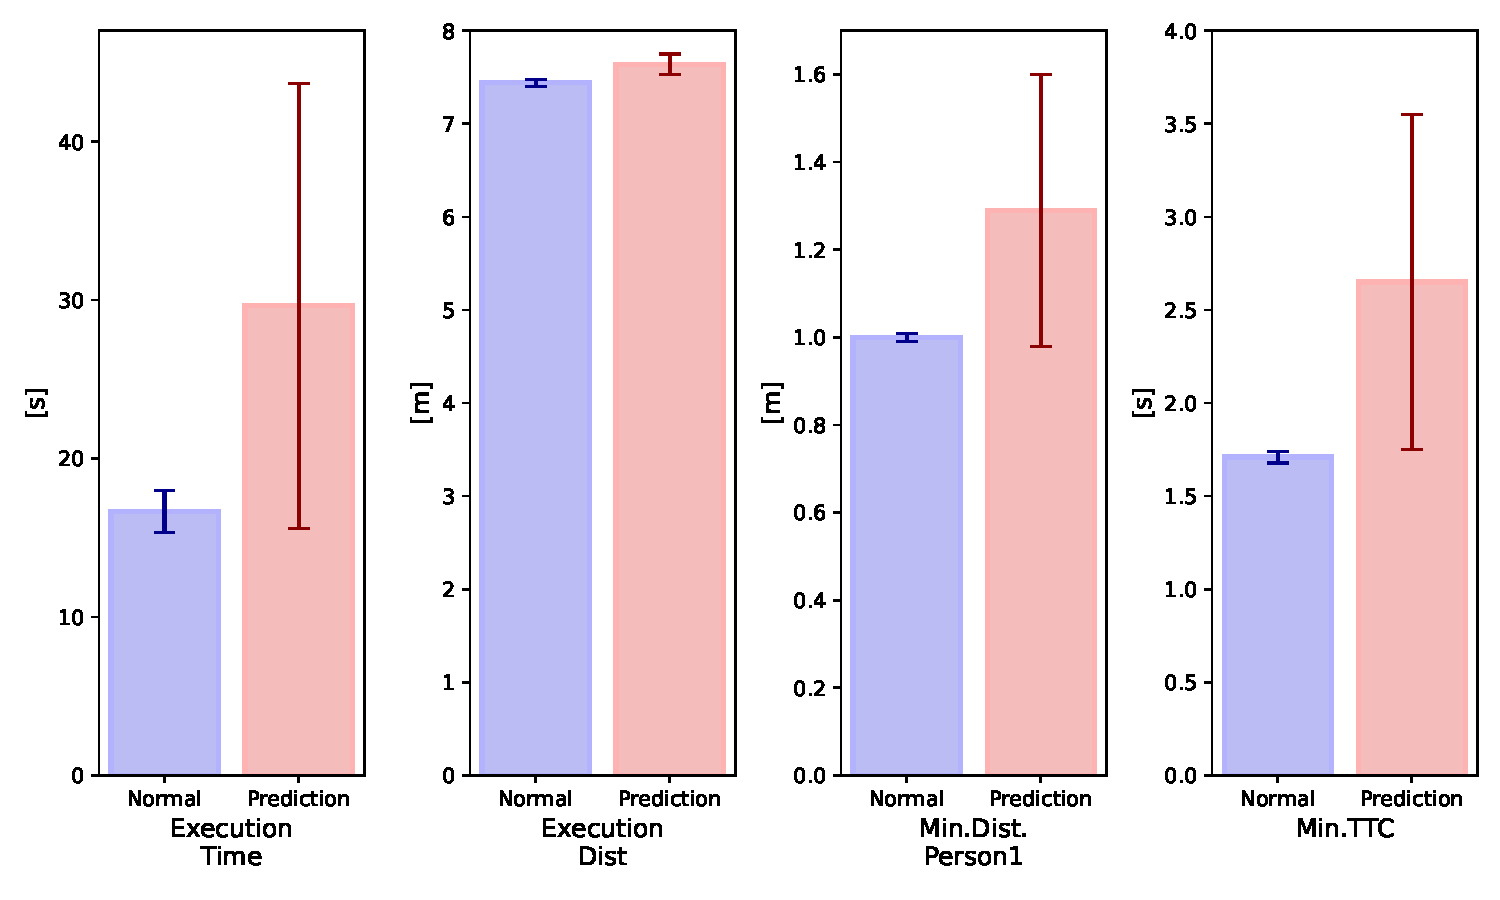
\includegraphics[keepaspectratio, scale=0.53]
      {images/scenario1_result.pdf}
  \caption{Scenario1 result}
 \label{Fig:scenario1-result}
\end{figure} 

\newpage

\vspace*{20pt}
\begin{figure}[H]
  \centering
 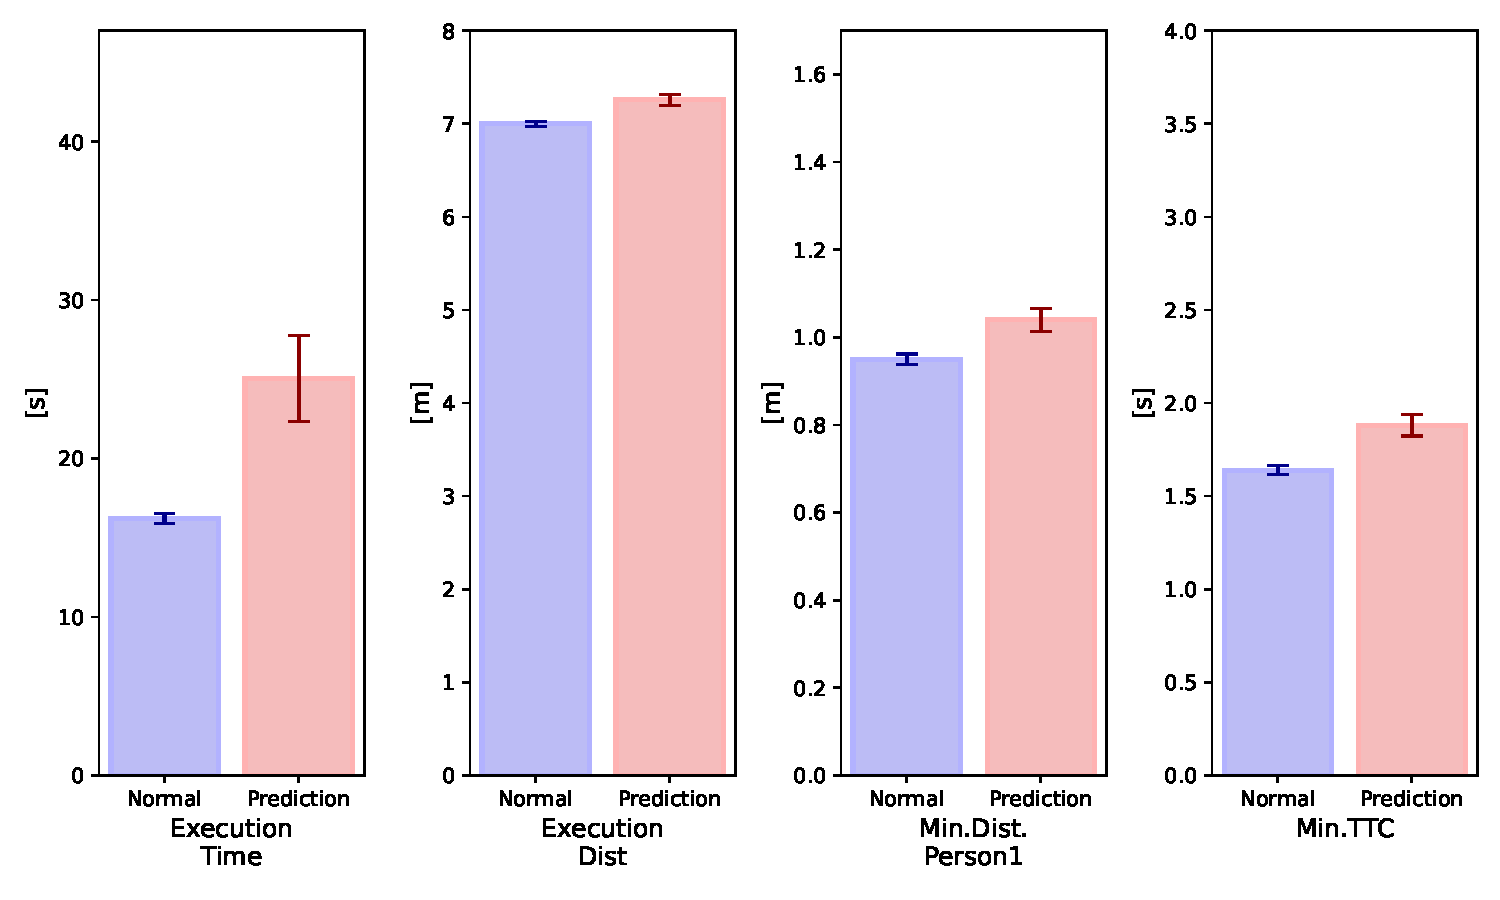
\includegraphics[keepaspectratio, scale=0.53]
      {images/scenario2_result.pdf}
  \caption{Scenario2 result}
 \label{Fig:scenario2-result}
\end{figure} 

\begin{figure}[H]
  \centering
 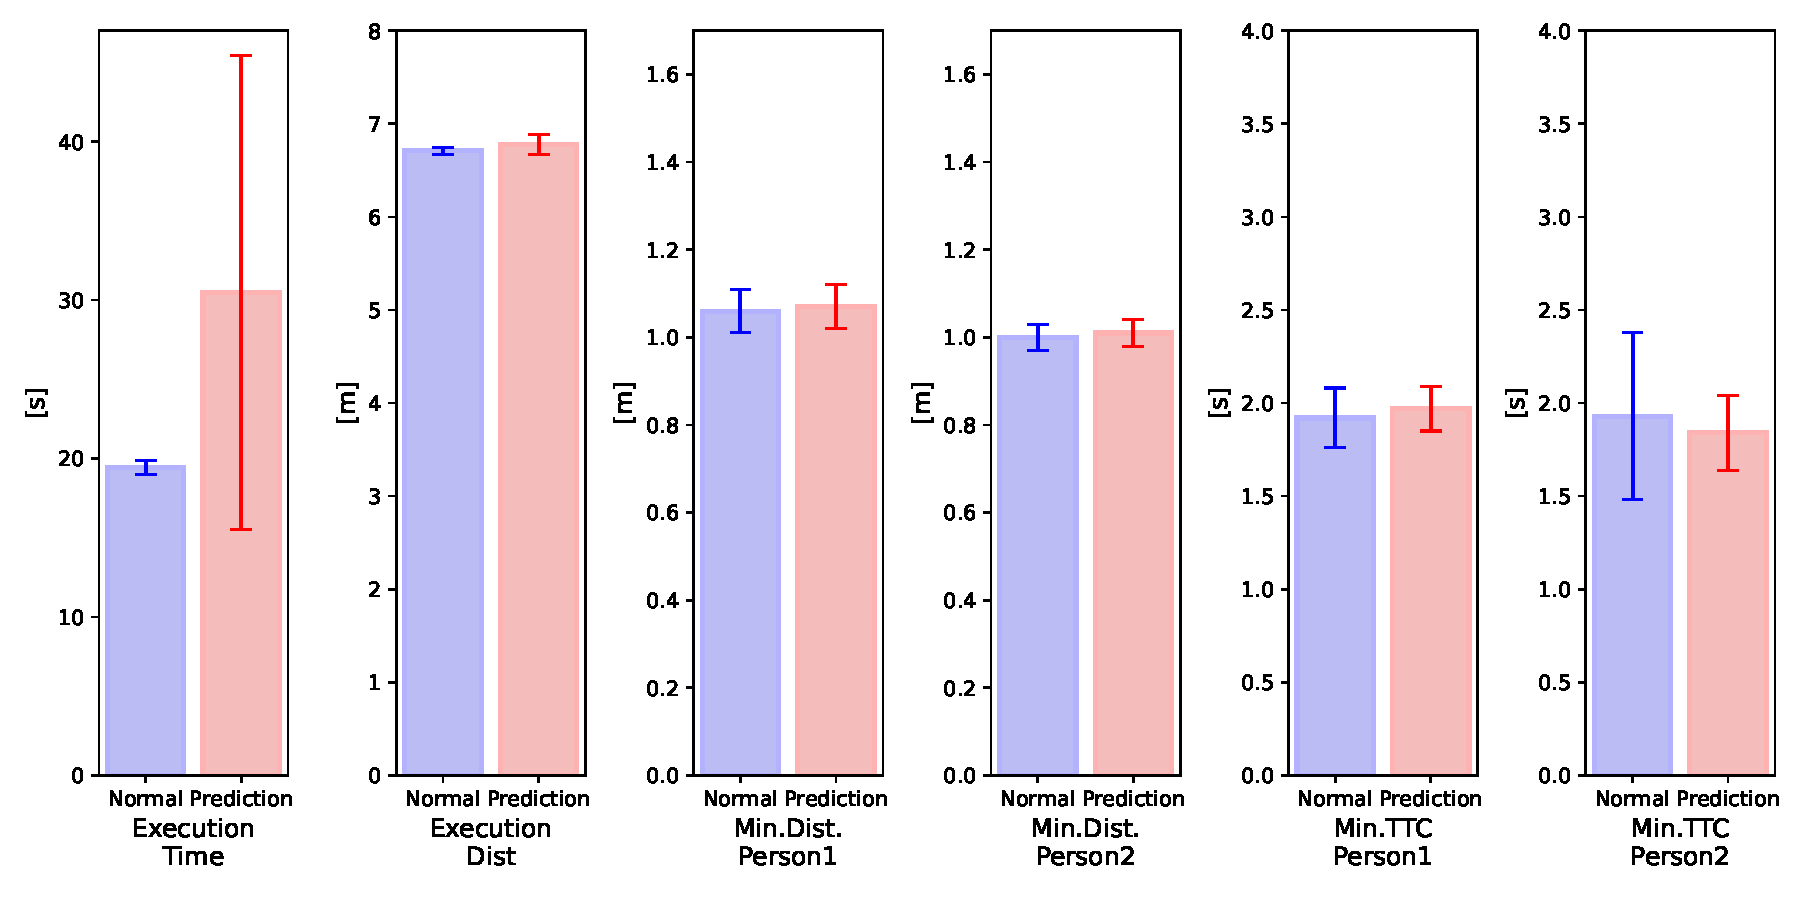
\includegraphics[keepaspectratio, scale=0.44]
      {images/scenario3_result.pdf}
  \caption{Scenario3 result}
 \label{Fig:scenario3-result}
\end{figure} 

\newpage

シナリオ1とシナリオ2では,歩行者との最小距離と最小TTCが改善されており,予測結果を活用することでロボットが早期に停止し,歩行者との接触リスクを低減できる可能性を示している.一方,停止や回避行動に伴い,走行時間・距離の増加が生じたと考えられる.
% 付録Aの\figref{Fig:cross-viz}および\figref{Fig:block-viz}には,ロボットと歩行者の位置の時間変化を可視化した例を示している.これらの図から,ロボットが早期に減速または停止を行う様子が確認できる.

シナリオ3では,歩行者1に対する最小距離と最小TTCが改善されているが,歩行者2との最小TTCが悪化している.これは,狭い通路ですれ違う際にロボットと歩行者2の接近速度が増加していることを意味している.この結果から,狭い空間など複雑なシナリオでのナビゲーションにおいては,予測結果の精度や活用方法のさらなる改善が必要と考えられる.また,本研究の学習に用いたデータセットはいずれも屋外の広い空間のデータであり,狭い環境に対する学習サンプルが不足していた点も影響したと考えられる.

本実験で用いたシミュレータの歩行者は,Social Force Model\cite{s-force-model}を用いてロボットや他の歩行者との相互作用を再現しているが,現実の歩行者の動きとは完全に一致しない.その結果,現実の歩行者の動きを重視して学習したモデルと実験環境の性質が乖離し,予測性能が低下した可能性がある.さらに,予測結果を用いる場合の標準偏差が大きい要因として,以下の点が考えられる.
% \vspace{-10pt}
\begin{itemize}
  \item 正規分布からサンプリングされた軌道が実際の軌道と大きく異なる場合がある
  \item 予測結果が更新される際にロボットの経路計画にチャタリングを引き起こす(\figref{Fig:sequences})
  \item 前後の予測結果(例えば,$t-1\text{と}t$)に一貫性がない場合がある
\end{itemize}
% \vspace{-10pt}
これらの課題を解決するためには,狭い空間など多様な環境,相互作用を含むデータセットの活用や,提案したナビゲーションシステムの予測結果の活用方法の改善などが必要になると考えられる.

\begin{figure}[H]
  \centering
  \begin{subfigure}{\linewidth}
    \centering
    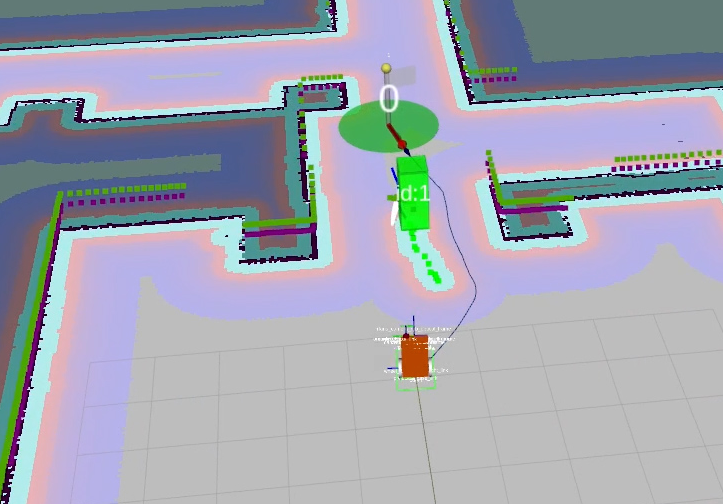
\includegraphics[keepaspectratio, scale=0.28]{images/seq-19.png}
    \caption{t = 0}
    \label{Fig:seq-19}
  \end{subfigure}
  
  % \vspace{10pt}
  
  \begin{subfigure}{\linewidth}
    \centering
    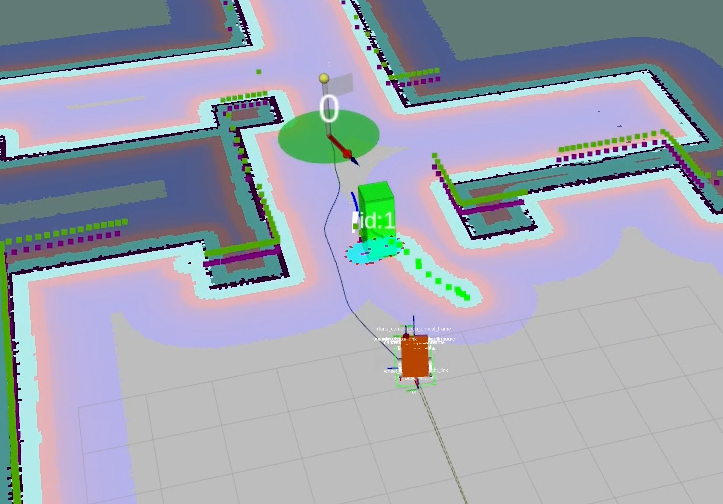
\includegraphics[keepaspectratio, scale=0.28]{images/seq-20.png}
    \caption{t = 1}
    \label{Fig:seq-20}
  \end{subfigure}
  
  % \vspace{10pt}
  
  \begin{subfigure}{\linewidth}
    \centering
    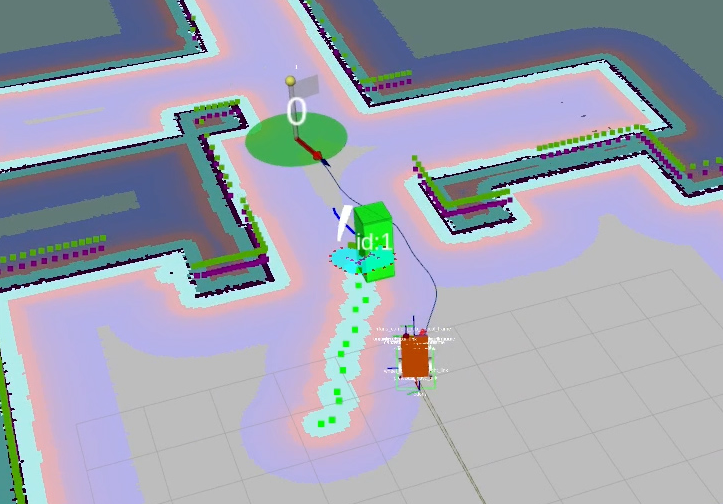
\includegraphics[keepaspectratio, scale=0.28]{images/seq-21.png}
    \caption{t = 2}
    \label{Fig:seq-21}
  \end{subfigure}
  
  % \vspace{-10pt}
  
  \caption{\centering Chattering in robot path planning due to updating prediction results \newline (t represents time in seconds, with one-second intervals)}
  \label{Fig:sequences}
\end{figure}

\newpage
